\chapter{균질 공간의 기하학}

\lectureoverview{평탄성은 관측된 우주를 매우 잘 근사하지만, 원리는 아니다. 곡률을 허용하면서 균질성과 등방성을 유지하면, 단일 연결 공간 기하 세 가지가 나온다. 유클리드 공간, 구면 공간, 쌍곡 공간이다. 이들의 계량은 동심 껍질이 거리에 따라 어떻게 커지는지를 통해 구성할 수 있으며, 각크기와 천체 수를 이용해 곡률을 검증할 수 있다. 위상 공간이 토러스형이면 평탄 공간도 유한할 수 있다. 마지막으로 이러한 균질 공간 중 어느 것이든 시간에 따라 변하는 척도인자를 붙이면 우주론적 시공간 계량과 허블 법칙을 얻는다. 이 척도인자의 동역학은 일반상대성이론에서 나와야 한다.}

\section{평탄성은 관측 사실이지 원리가 아니다}

지금까지 우리는 공간을 평탄하다고 보고 시공간의 기하학에 대해서는 거의 다루지 않았다. 관측에 따르면 평탄 공간은 매우 좋은 근사이지만, 그렇다고 평탄성이 법칙이 되는 것은 아니다. 측정으로 실제 알 수 있는 것은 곡률반지름이 우리가 조사한 영역보다 훨씬 커야 한다는 점이다. 공간은 정확히 평탄할 수도 있고, 양의 곡률이나 음의 곡률을 가질 수도 있다. 관측 가능한 영역을 훨씬 넘어선 규모에서 어느 설명이 맞는지는 아직 모른다.

따라서 한 가지 가정은 완화하되 다른 가정은 유지하겠다. 평탄성을 가정하지는 않지만, 공간이 균질하고 등방적이라는 가정은 계속 두겠다. 이는 신념의 조항이 아니라 작업 가설이다. 그 결과를 알아보기 위해 이를 가정하고 계산한 뒤, 이 가정을 버리고 비균질 우주에서는 무엇이 달라지는지 물을 수 있다.

균질성이란 모든 점이 기하학적으로 같은 성격을 가진다는 뜻이다. 다른 곳으로 옮겨 가서 국소적인 기하 실험을 되풀이하는 관측자도 같은 결과를 얻는다. 등방성이란 특별히 선호되는 방향이 없다는 뜻이다. 이 조건을 적용하면 처음 떠올리기 쉬운 곡면 대부분은 배제된다. 포물면은 꼭짓점 부근에서 멀리 떨어진 곳보다 더 급하게 휘어 있다. 긴 타원체는 극과 허리 부분이 서로 다르다. 울퉁불퉁한 구나 산과 계곡까지 분해해 본 지표면은 휘어 있지만 균질하지 않다. 우주론에서 묻는 것은 더 제한적이다:
\begin{quote}
모든 점과 모든 방향에서 기하학적으로 똑같이 보이면서 휘어 있을 수 있는 공간은 무엇인가?
\end{quote}

전역적인 동일시를 잠시 무시하면, 상수 곡률을 가진 답은 세 가지다. 평탄 공간, 양의 곡률을 가진 구면 공간, 음의 곡률을 가진 쌍곡 공간이다. 전역적 동일시에 관한 단서는 중요하다. 뒤에서 평탄하고 유한한 토러스를 구성해, 이 세 공간이 모든 가능성을 빠짐없이 포괄한다는 지나치게 단순한 주장을 바로잡겠다.

\section{계량과 관측자의 좌표}

먼저 시공간이 아니라 공간만 논하자. 공간의 기하학은 계량, 즉 이웃한 두 점 사이의 제곱 거리 \(ds^2\)를 정하는 규칙으로 표현된다. 이 국소 규칙을 모든 곳에서 알면 길이, 각도, 면적, 부피, 측지선과 곡률을 모두 구할 수 있다.

유클리드 평면과 유클리드 삼차원 공간에서는 데카르트 좌표로 다음과 같이 쓴다.
\begin{equation}
ds_2^2=dx^2+dy^2,
\qquad
ds_3^2=dx^2+dy^2+dz^2.
\label{eq:c03-cartesian-flat}
\end{equation}
세 번째 차원을 더하면 직교하는 항 \(dz^2\)만 추가된다. 그러나 중요한 점은 이 식이 간단하다는 데 있지 않다. 방정식~\eqref{eq:c03-cartesian-flat}이 국소 기하학을 완전히 규정한다는 데 있다.

\begin{figure}[htbp]\centering
\includegraphics[width=0.74\textwidth]{lecture_03_figure_02.png}\caption{칠판에 적힌 평탄한 삼차원 공간의 데카르트 계량.}\label{fig:c03-cartesian-board}\lectureframe{00:05:13.138}\end{figure}

데카르트 좌표로는 천문학자가 우주를 경험하는 방식이 잘 드러나지 않는다. 우리는 한 점에 자리 잡고 방향을 따라 바깥을 바라보며, 보이는 것을 각도와 거리에 따라 분류한다. 우주가 이차원이라면 시야는 말 그대로 우리 주위의 방향들로 이루어진 원이 될 것이다. 따라서 극좌표는 단지 우아한 좌표계가 아니다. 우주론에서 쓰이는 각도 기하학을 드러내 준다.

반지름 방향 거리를 \(r\), 방향을 \(\theta\)라 하자. 같은 유클리드 평면의 계량은 이제 다음과 같다.
\begin{equation}
ds^2 = dr^2 + r^2 d\theta^2.
\label{eq:c03-polar-flat}
\end{equation}
작은 각 \(d\theta\)가 고정되어 있으면, 횡방향 간격은 \(r\,d\theta\)이다. 바깥쪽으로 이동할수록 이 간격은 선형으로 커지므로, 계량에 기여하는 그 제곱 항은 \(r^2d\theta^2\)가 된다.

각도 항 자체도 일차원 공간의 계량이다. 원은 일구면이라 하며 \(S^1\)로 표기한다. 단위원의 계량은 관례적으로 다음과 같이 쓴다.
\begin{equation}
d\Omega_1^2 = d\theta^2,
\qquad\text{so that}\qquad
ds^2 = dr^2 + r^2 d\Omega_1^2.
\label{eq:c03-omega-one}
\end{equation}
칠판에는 읽을 수 있는 아래첨자 없이 \(d\Omega^2\)가 적혀 있지만, 구두 설명에 따르면 의도된 대상은 \(d\Omega_1^2\)이다.

\begin{figure}[htbp]\centering
\includegraphics[width=0.74\textwidth]{lecture_03_figure_03.png}\caption{평탄 공간의 극좌표 스케치와 계량. 칠판에는 \(d\Omega^2\)가 적혀 있고, 설명에서는 이를 단위원의 계량 \(d\Omega_1^2=d\theta^2\)로 확인한다.}\label{fig:c03-polar-board}\lectureframe{00:08:37.254}\end{figure}

\begin{figure}[htbp]\centering
\begin{tikzpicture}[scale=1.2]
\draw[->] (-1.2,0)--(1.8,0);
\draw[->] (0,-1.2)--(0,1.8);
\draw[thick] (0,0)--(1.3,1.1);
\draw (0.7,0.7) node[above] {$r$};
\draw (0.58,0) arc (0:40:0.58);
\draw (0.8,0.22) node {$\theta$};
\end{tikzpicture}\caption{방정식~\eqref{eq:c03-omega-one}에서 사용하는 관측자 중심 극좌표를 깔끔하게 다시 그린 그림.}\label{fig:c03-polar-redraw}\end{figure}

\begin{classroomqa}\audiencequestion{\(d\theta^2\)는 실제로 원주를 따라 잰 거리를 나타내나요?}\lecturerresponse{그렇다. 단위원에서는 호의 길이가 라디안 단위의 각도와 같으므로, \(d\theta\)만큼 떨어진 이웃한 점 사이의 내재적 거리의 제곱은 \(d\theta^2\)이다. 원주의 길이는 \(2\pi\)이며, 이를 따라 \(ds=d\theta\)를 한 바퀴 적분하면 정확히 \(2\pi\)이 된다. 여기에 \(r^2\)를 곱하면 단위원이 평면에서 반지름 \(r\)인 껍질로 커진다. \lecturetimestamp{00:09:11--00:09:26}}\end{classroomqa}

\emph{내재적}이라는 말이 중요하다. 단위원을 유클리드 평면에 놓으면 다음과 같이 표현할 수 있다.
\begin{equation}
x^2 + y^2 = 1.
\end{equation}
이 방정식은 원이 더 큰 공간 안에 어떻게 놓여 있는지를 설명한다. 원 위에서 거리만 잴 수 있는 거주자에게는 이 식이 필요하지 않다. 유연한 광섬유를 늘이지 않고 구불구불한 닫힌 고리 모양으로 구부릴 수 있다. 평면에서 보이는 모양은 바뀌겠지만, 내재적 원주 길이와 계량은 그대로다. \(\theta\)를 같은 만큼 늘릴 때마다 광섬유를 따라 잰 거리도 여전히 같게 늘어난다. 따라서 기하학은 매장으로 인해 우연히 주어진 모양과 구분해야 한다.

\begin{figure}[htbp]\centering
\includegraphics[width=0.64\textwidth]{lecture_03_figure_04.png}\caption{칠판은 둥근 단위원과 변형된 닫힌 고리를 비교한다. 늘이지 않고 고리를 구부리면 두 도형의 내재적인 일차원 계량은 같다.}\label{fig:c03-intrinsic-board}\lectureframe{00:10:34.205}\end{figure}

\begin{figure}[htbp]\centering
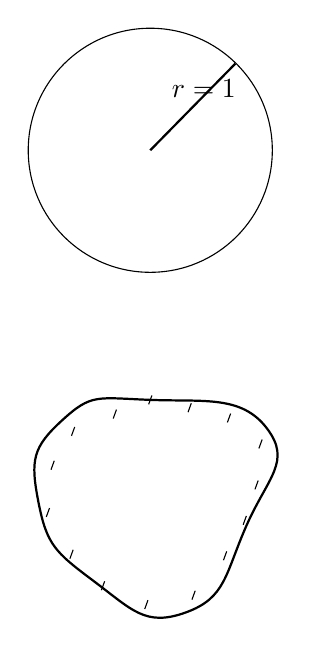
\begin{tikzpicture}[scale=1.0]
\draw (0,0) circle (1.55);
\draw[thick] (0,0)--(1.08,1.1);
\draw (0.68,0.78) node {$r=1$};

\begin{scope}[yshift=-4.35cm]
\draw[thick]
plot[smooth cycle, tension=0.95] coordinates
{(0,1.18) (1.48,0.82) (1.22,-0.42) (0.45,-1.52) (-0.72,-1.12) (-1.42,-0.12) (-1.12,0.92)};
\foreach \p in {(0,1.18),(0.5,1.08),(1.0,0.95),(1.4,0.62),(1.35,0.1),(1.2,-0.35),(0.95,-0.8),(0.55,-1.3),(-0.05,-1.42),(-0.6,-1.18),(-1.0,-0.78),(-1.3,-0.25),(-1.24,0.35),(-0.98,0.78),(-0.45,1.0)}{
\draw[rotate around={70:\p}] \p ++(-0.06,0) -- ++(0.12,0);
}
\end{scope}
\end{tikzpicture}\caption{외재적 변형을 거쳐도 내재적 거리는 유지된다. 일차원 공간의 거주자는 어느 쪽에 매장해도 같은 원주 길이를 잰다.}\label{fig:c03-intrinsic-redraw}\end{figure}

이제 평탄 공간을 관측자를 중심으로 동심원을 겹겹이 쌓은 것으로 볼 수 있다. 거리 \(r\)에 있는 껍질은 단위원을 \(r\)만큼 확대한 것이다. 이것이 바로 인자 \(r^2d\Omega_1^2\)가 나타내는 내용이다.

\section{양의 곡률: 닫히는 껍질}

구면은 휘어 있지만 균질하다. 완벽한 구면에는 다른 점과 기하학적으로 구별되는 점이 없다. 외부의 삼차원 그림에 기대지 않고도 구면의 계량을 구성할 수 있다. 단위 \(2\)-구면에 사는 이차원 천문학자들을 생각하고, 그들이 각자 있는 곳에 좌표의 원점을 둔다고 하자.

이 천문학자들을 둘러싼 작은 측지 거리 \(r\)의 원은 작다. \(r\)가 커지면 원들도 커져 구면을 반 바퀴 돈 곳에서 원주가 최대가 되고, 그 뒤에는 줄어들어 대척점에서 한 점으로 수축한다. 이 성장과 수축은 시간에 따른 것이 아니라 \emph{거리}에 따른 것이다. 이 구성에서 구면은 내내 정지해 있다.

여기서 \(r\)은 중심으로부터의 유클리드 거리가 아니라 단위 구면을 따른 각거리다.
\[
0 \le r \le \pi.
\]
\(r=0\)은 선택한 원점이고, \(r=\pi/2\)에는 반대편 대원이 있으며, \(r=\pi\)에는 대척점이 있다. 이제 껍질의 반지름은 \(\sin r\)이므로, 평탄 공간의 인자 \(r^2\)는 \(\sin^2r\)로 바뀐다.
\begin{equation}
d\Omega_2^2 = dr^2 + \sin^2 r\, d\Omega_1^2
            = dr^2 + \sin^2 r\, d\theta^2.
\label{eq:c03-two-sphere}
\end{equation}
양 끝점과 중간점은 필요한 대로 거동한다.
\begin{equation}
\sin 0=0,
\qquad
\sin\frac{\pi}{2}=1,
\qquad
\sin\pi=0.
\end{equation}
따라서 껍질은 크기 0에서 시작해 최대 크기에 도달한 뒤 다시 닫힌다.

\begin{figure}[htbp]\centering
\includegraphics[width=0.82\textwidth]{lecture_03_figure_05.png}\caption{평탄 공간의 동심원에서 구면의 껍질로 이어지는 변화. 아래쪽 식은 영상에서 일부 가려져 있지만, 구두 유도에 따르면 방정식~\eqref{eq:c03-two-sphere}에서 \(r^2\mapsto\sin^2r\)로 바뀐다.}\label{fig:c03-spherical-board}\lectureframe{00:16:11.701}\end{figure}

\begin{figure}[htbp]\centering
\resizebox{\linewidth}{!}{%
\begin{tikzpicture}[scale=0.92]
\begin{scope}[xshift=-4.15cm]
\draw[->] (-1.7,0)--(1.9,0);
\draw[->] (0,-1.7)--(0,1.9);
\draw (0,0) circle (0.45);
\draw (0,0) circle (0.9);
\draw (0,0) circle (1.35);
\draw[thick] (0,0)--(1.45,1.2);
\draw (0.56,0.18) arc (18:40:0.63);
\draw (0.94,0.44) node {$\theta$};
\end{scope}

\begin{scope}[xshift=4.15cm]
\draw (0,0) circle (2.0);
\fill (0,-2.0) circle (1.5pt);
\fill (2.0,0) circle (1.5pt);
\fill (0,2.0) circle (1.5pt);
\draw[thick] (0,-2.0) arc (-90:90:2.0);
\draw (0,-2.35) node {$r=0$};
\draw (2.75,0) node {$r=\pi/2$};
\draw (0,2.35) node {$r=\pi$};
\end{scope}
\end{tikzpicture}}%
\caption{평탄 공간의 껍질은 계속 커지지만, 구면의 껍질은 \(r=\pi/2\)에서 최대 크기에 이른 뒤 \(r=\pi\)에서 닫힌다.}\label{fig:c03-shells-flat-sphere}\end{figure}

표기 \(d\Omega_2^2\)는 단위 \(2\)-구면의 계량을 뜻하며, \(d\Omega_1^2\)가 그 원형 껍질의 계량을 뜻하는 것과 같다. 같은 재귀적 구성은 차원을 하나 높여도 성립한다. 평탄한 삼차원 공간에서 고정된 반지름에 있는 우리 주위의 껍질은 \(2\)-구면이다.
\begin{equation}
ds_{\text{flat},3}^2 = dr^2 + r^2 d\Omega_2^2.
\label{eq:c03-flat-three-polar}
\end{equation}
이 \(2\)-구면 껍질들이 인자 \(\sin r\)에 따라 커졌다가 닫히면, 결과 공간은 단위 \(3\)-구면이 된다.
\begin{equation}
d\Omega_3^2 = dr^2 + \sin^2 r\, d\Omega_2^2.
\label{eq:c03-three-sphere}
\end{equation}
\(3\)-구면은 익숙한 매장을 나타내려면 유클리드 사차원 공간이 필요하므로 그리기 어렵다. 그러나 계량은 완전하며 그림을 필요로 하지 않는다. 선택한 관측자 주위에 \(2\)-구면들이 겹겹이 놓이고, 이들은 최대 크기까지 커진 뒤 대척점을 향해 줄어든다.

\begin{classroomqa}\audiencequestion{관측자는 구면의 중심에 있나요?}\lecturerresponse{관측자는 \emph{좌표 껍질}의 중심에 있을 뿐, 기하학적으로 특별한 중심에 있는 것은 아니다. 원점은 공간 위의 한 점이며, 다른 관측자도 자기 위치를 \(r=0\)로 정해 똑같은 계량을 얻을 수 있다. 바로 그런 선택 중 어느 것도 우선되지 않는다는 것이 균질성의 뜻이다. \lecturetimestamp{00:19:21--00:20:27}}\end{classroomqa}

시각화만을 위해 단위원과 단위 \(2\)-구면을 유클리드 공간에 매장할 수 있다.
\begin{equation}
x^2+y^2=1,
\qquad
x^2+y^2+z^2=1.
\end{equation}
이 식들은 매장을 나타낼 뿐, 추가적인 물리학을 뜻하지는 않는다. 원이나 구면에만 갇힌 개미도 주위의 유클리드 공간을 감지하지 않고 내재적 계량을 알아낼 수 있다. 마찬가지로 \(S^3\)는 알 수 없는 경계가 있는 평범한 공이 아니다. 방정식~\eqref{eq:c03-three-sphere}이 기술하는 완전한 삼차원 공간이다.

\section{곡률이 관측에 미치는 영향}

기하학이 관측에 변화를 일으킬 때 비로소 물리학이 된다. 횡방향 지름이 알려진 물체 \(d\)가 있고, 그 반지름 방향 거리 \(r\)는 독립적으로 추론했으며, 하늘에서의 각지름 \(d\theta\)을 측정했다고 하자. 은하가 대략적인 직관의 예가 되지만, 정밀한 우주론에서는 보정된 표준자와 표준광원을 사용한다. 거리 정보는 스펙트럼 적색편이, 허블 관계, 광도와 서로 다른 천체 종류 사이의 교차 보정을 통해 종합할 수 있다.

평탄 공간에서는 물체의 횡방향 너비를 가로질러 \(r\)를 고정한다. 방정식~\eqref{eq:c03-polar-flat}에 따르면
\begin{equation}
d^2 = r^2 d\theta^2.
\label{eq:c03-flat-angle-step}
\end{equation}
따라서
\begin{equation}
d\theta = \frac{d}{r}.
\label{eq:c03-flat-angle}
\end{equation}
각크기는 거리에 반비례해 작아진다.

단위 구면에서는 횡방향 껍질의 크기가 \(r\)가 아니라 \(\sin r\)이다.
\begin{equation}
d^2 = \sin^2 r\, d\theta^2,
\qquad\text{hence}\qquad
d\theta = \frac{d}{\sin r}.
\label{eq:c03-spherical-angle}
\end{equation}
\(0<r<\pi\)일 때 \(\sin r<r\)이므로, 같은 거리에 있는 같은 물체는 평탄 공간에서보다 더 크게 보인다. 각크기는 처음에는 작아지다가 적도에서 최소가 되고, 껍질이 수축하면서 다시 커진다. 대척점에서는 모든 방향이 한데 모여 영상이 하늘을 가득 채우는 것이 이상적인 극한에서의 결과다.

\begin{classroomqa}\audiencequestion{우주배경복사를 이용해 곡률을 추론하는 것도 같은 발상인가요?}\lecturerresponse{그렇다. 초기 플라스마의 음향 진동이 특징적인 물리적 척도를 제공한다. 우리는 그 표준자의 각크기를 측정하고 각 기하학이 예측하는 각도와 비교한다. 대상이 반드시 은하일 필요는 없다. 핵심은 알려진 횡방향 척도와 관측된 각크기를 비교하는 것이다. \lecturetimestamp{00:37:37--00:38:12}}\end{classroomqa}

껍질 부피는 두 번째 검증 방법을 제공한다. 평탄한 삼차원 공간에서 껍질의 면적은 \(r^2\)에 비례하고, 단위 \(3\)-구면에서는 \(\sin^2r\)에 비례한다. 따라서 균질한 분포에서는 구면 껍질 위의 천체 수가 처음에는 거리에 따라 증가하다가 적도 이후에는 감소한다. 양의 곡률은 평탄 공간과 비교해 짝을 이루는 신호를 예측한다. 충분히 먼 표준자는 지나치게 크게 보이고, 먼 껍질에는 천체가 너무 적다.

\begin{figure}[htbp]\centering
\resizebox{\linewidth}{!}{%
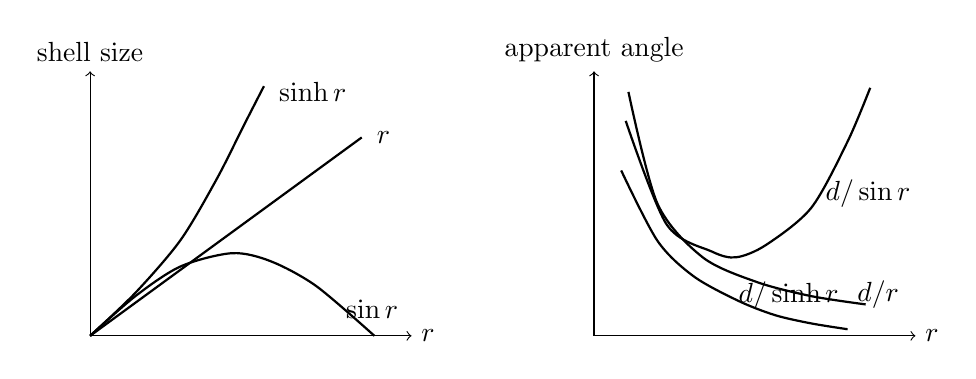
\begin{tikzpicture}[x=1.15cm,y=1.05cm]
\begin{scope}
\draw[->] (0,0)--(3.55,0) node[right] {$r$};
\draw[->] (0,0)--(0,3.2) node[above] {shell size};

\draw[thick] (0,0)--(3.0,2.4);
\draw (3.06,2.4) node[right] {$r$};

\draw[thick]
plot[smooth] coordinates {(0,0) (0.5,0.48) (1.0,0.84) (1.57,1.0) (2.0,0.9) (2.5,0.6) (3.14,0)};
\draw (2.72,0.55) node[below right] {$\sin r$};

\draw[thick]
plot[smooth] coordinates {(0,0) (0.5,0.52) (1.0,1.16) (1.4,1.9) (1.7,2.55) (1.92,3.02)};
\draw (1.98,2.95) node[right] {$\sinh r$};
\end{scope}

\begin{scope}[xshift=6.4cm]
\draw[->] (0,0)--(3.55,0) node[right] {$r$};
\draw[->] (0,0)--(0,3.2) node[above] {apparent angle};

\draw[thick]
plot[smooth] coordinates {(0.38,2.95) (0.7,1.6) (1.2,0.95) (1.8,0.65) (2.4,0.48) (3.0,0.38)};
\draw (2.8,0.5) node[right] {$d/r$};

\draw[thick]
plot[smooth] coordinates {(0.35,2.6) (0.8,1.35) (1.3,1.02) (1.57,0.95) (1.9,1.1) (2.4,1.55) (2.8,2.35) (3.05,3.0)};
\draw (2.45,1.72) node[right] {$d/\sin r$};

\draw[thick]
plot[smooth] coordinates {(0.3,2.0) (0.7,1.15) (1.1,0.72) (1.6,0.42) (2.0,0.25) (2.4,0.15) (2.8,0.08)};
\draw (2.15,0.2) node[above] {$d/\sinh r$};
\end{scope}
\end{tikzpicture}}%
\caption{방사형 껍질 인자와 그에 대응하는 각크기 법칙. 양의 곡률에서는 껍질이 닫히고, 음의 곡률에서는 껍질이 지수적으로 커진다.}\label{fig:c03-shell-angular-laws}\end{figure}

\begin{classroomqa}\audiencequestion{구면을 계속 돌아가면 방사형 좌표가 무한대가 되나요?}\lecturerresponse{아니다. 단위 구면에서 \(r\)는 측지 각거리이며, 범위는 \(0\)부터 \(\pi\)까지뿐이다. \(r=\pi\)에서는 대척점에서 껍질이 수축해 사라진다. 여기서 살펴보는 것은 고정된 공간 기하학이지, 시간에 따라 바깥쪽으로 움직이는 물체가 아니다. 뒤에서 곡률반지름을 도입하면 모든 물리적 거리에 그 반지름을 곱하지만, 이 무차원 범위는 달라지지 않는다. \lecturetimestamp{00:39:30--00:40:35}}\end{classroomqa}

\section{사영은 기하학이 아니다}

음의 곡률로 넘어가기 전에, 충실한 기하학도 그림으로 나타내면 얼마나 심하게 왜곡될 수 있는지 살펴보자. 구면을 남극에서 접하는 평면 위에 놓는다. 북극에서 구면의 각 점 \(P\)을 지나는 직선을 그어 평면까지 연장하고, 평면과 만나는 점을 \(P'\)이라 하자. 이것이 입체 사영이다. 북극 자체는 무한대로 보내진다. 남극 근처의 작은 영역은 거의 왜곡 없이 표현되지만, 북극 근처의 같은 내재적 크기의 영역은 평면에서 엄청나게 커진다.

왜곡은 구면이 아니라 사상에 속한다. 평면에 그린 모습에서 서로 동등한 영역의 좌표 크기가 크게 달라져도, 원래 구면은 여전히 균질하다. 무한한 쌍곡 공간을 유한한 원판에 압축할 때도 이 점을 염두에 두어야 한다.

\begin{figure}[htbp]\centering
\resizebox{\linewidth}{!}{%
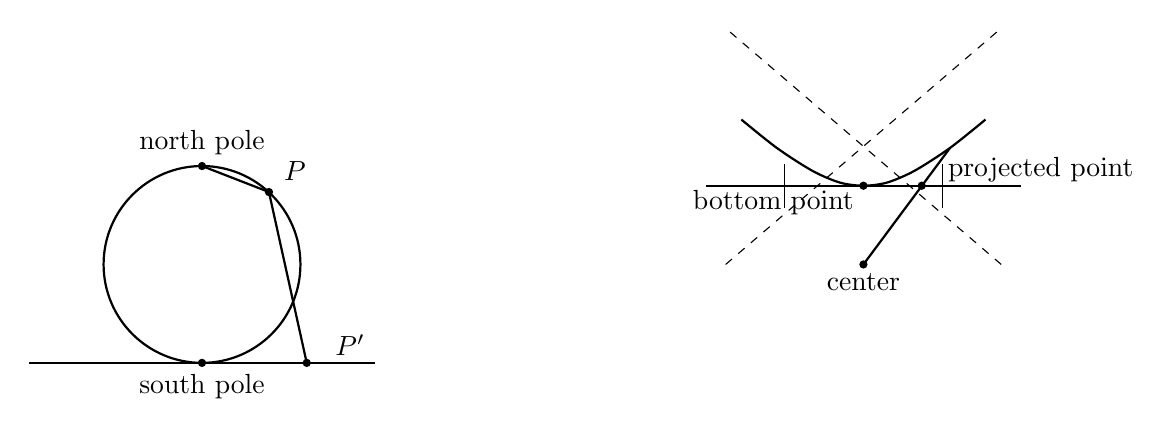
\begin{tikzpicture}[scale=1.0]
\begin{scope}[xshift=-4.2cm]
\draw[thick] (-2.2,-1.25)--(2.2,-1.25);
\draw[thick] (0,0) circle (1.25);
\fill (0,1.25) circle (1.5pt);
\fill (0,-1.25) circle (1.5pt);
\draw (0,1.55) node {north pole};
\draw (0,-1.55) node {south pole};

\fill (0.85,0.92) circle (1.5pt);
\draw (0.92,1.18) node[right] {$P$};
\draw[thick] (0,1.25)--(0.85,0.92)--(1.33,-1.25);
\fill (1.33,-1.25) circle (1.5pt);
\draw (1.57,-1.03) node[right] {$P'$};
\end{scope}

\begin{scope}[xshift=4.2cm]
\draw[thick] (-2.0,1)--(2.0,1);
\draw[dashed] (-1.75,0)--(1.75,3.0);
\draw[dashed] (1.75,0)--(-1.75,3.0);
\draw[thick]
plot[smooth] coordinates
{(-1.55,1.84) (-1.1,1.48) (-0.65,1.19) (-0.3,1.04) (0,1.0) (0.3,1.04) (0.65,1.19) (1.1,1.48) (1.55,1.84)};
\fill (0,0) circle (1.5pt);
\fill (0,1) circle (1.5pt);
\draw (0,-0.22) node {center};
\draw (0,0.78) node[left] {bottom point};
\draw[thick] (0,0)--(1.1,1.48);
\fill (0.74,1.0) circle (1.5pt);
\draw (0.95,1.2) node[right] {projected point};
\draw (-1,0.72) -- (-1,1.28);
\draw (1,0.72) -- (1,1.28);
\end{scope}
\end{tikzpicture}}%
\caption{왼쪽: 구면의 북극을 무한대로 보내는 입체 사영. 오른쪽: 쌍곡면을 유한한 원판에 사영했다. 여기서는 단면인 선분으로 나타냈다. 좌표의 왜곡은 내재적 균질성을 깨뜨리지 않는다.}\label{fig:c03-projections}\end{figure}

\section{음의 곡률: 평탄 공간보다 더 빠르게 커지는 껍질}

세 번째 단일 연결 균질 기하학에서는 \(\sin r\)가 쌍곡 사인으로 바뀐다. 이차원과 삼차원에서 단위 계량은 다음과 같다.
\begin{equation}
dh_2^2 = dr^2 + \sinh^2 r\, d\Omega_1^2,
\label{eq:c03-hyperbolic-two}
\end{equation}
\begin{equation}
dh_3^2 = dr^2 + \sinh^2 r\, d\Omega_2^2.
\label{eq:c03-hyperbolic-three}
\end{equation}
이제 좌표 \(r\)의 범위는 다음과 같다.
\begin{equation}
0\le r<\infty.
\end{equation}
원점 근처에서는 \(\sinh r\approx r\)이므로 기하학은 국소적으로 유클리드적이다. 멀리 떨어진 곳에서는 껍질이 유클리드 껍질보다 훨씬 빠르게 커지며, 방향을 바꾸어 다시 줄어들지 않는다.

성장 법칙은 다음 식에서 나온다.
\begin{equation}
\sin r = \frac{e^{ir}-e^{-ir}}{2i},
\qquad
\sinh r = \frac{e^r-e^{-r}}{2}.
\label{eq:c03-sin-sinh}
\end{equation}
큰 \(r\)에서는 \(\sinh r\sim e^r/2\)이다. 따라서 이차원에서 원주는 반지름에 따라 지수적으로 커지고, 삼차원에서 껍질 면적은 \(\sinh^2r\sim e^{2r}/4\)에 따라 커진다. 균질한 분포라면 먼 껍질에는 그에 상응해 많은 천체가 들어 있다.

크기가 \(d\)인 횡방향 물체에 대해
\begin{equation}
d^2 = \sinh^2 r\, d\theta^2,
\qquad\text{so}\qquad
d\theta = \frac{d}{\sinh r}.
\label{eq:c03-hyperbolic-angle}
\end{equation}
큰 \(r\)에서는
\begin{equation}
d\theta \sim 2d\,e^{-r}.
\end{equation}
따라서 음의 곡률은 양의 곡률과 반대되는 신호를 보인다. 먼 표준자는 너무 작게 보이고, 먼 껍질에는 평탄 공간의 경우보다 천체가 너무 많다.

\begin{classroomqa}\audiencequestion{반지름 방향 좌표의 범위는 구면 공간과 쌍곡 공간을 어떻게 구분하나요?}\lecturerresponse{단위 구면에서는 \(r\)가 대척점 \(r=\pi\)에서 멈춘다. 쌍곡 공간에서는 \(0\le r<\infty\)처럼 한계 없이 계속된다. 껍질 인자도 같은 차이를 보여 준다. \(\sin r\)는 다시 0으로 돌아가지만, \(\sinh r\)는 끝없이 증가한다. \lecturetimestamp{00:52:46--00:53:25}}\end{classroomqa}

균질성을 이해하기 쉽게 해 주는 매장이 있다. 주변 공간의 좌표 \(T,x,y\)를 도입하자. 여기서 \(T\)는 매장 좌표일 뿐이며 우주론적 시간이 \emph{아니다}. 그리고 위쪽 시트를 취한다.
\begin{equation}
T^2 - x^2 - y^2 = 1.
\label{eq:c03-hyperboloid}
\end{equation}
주변 공간에 로런츠 부호 규약의 계량을 부여한다.
\begin{equation}
d\ell_{\mathrm{emb}}^2=-dT^2+dx^2+dy^2.
\label{eq:c03-ambient-minkowski}
\end{equation}
쌍곡면에 유도된 계량은 양의 정부호다. 로런츠 변환은 방정식~\eqref{eq:c03-hyperboloid}과~\eqref{eq:c03-ambient-minkowski}를 모두 보존하며, 위쪽 시트의 어느 점이든 다른 점으로 옮길 수 있다. 그런 의미에서 쌍곡 공간의 원점을 바꾸는 일은 보조 주변 공간에서 시간축을 기울이는 것과 같다. 모든 점은 기하학적으로 동등하다.

쌍곡면을 원판에 사영하면 무한히 먼 점들이 경계 원에 모인다. 가까운 영역은 거의 그대로 그려지지만, 멀리 있는 영역일수록 더 강하게 압축된다. 이것이 천사와 악마가 반복해서 그려지는 그림으로 잘 알려진 Poincar\'e 원판 표현이다. 좌표 변환으로 가장자리 부근의 작은 도형을 중심으로 옮기면 크게 만들 수 있으며, 이때 모든 내재적 길이와 각도는 보존된다. 삼차원에서는 이에 대응하는 모형이 원판이 아니라 공이다. \emph{Poincar\'e공간}, \emph{로바쳅스키 공간}, \emph{균일한 음의 곡률을 가진 공간}은 모두 같은 국소 기하학을 가리킨다.

\begin{classroomqa}\audiencequestion{유한 원판은 펜로즈 다이어그램과 비슷한가요?}\lecturerresponse{무한한 영역을 유한한 그림 안에 나타낸다는 제한된 의미에서는 비슷하다. 하지만 여기서 원판은 공간만을 나타내며, 시공간이나 인과적 무한대를 나타내지는 않는다. 그림에서는 경계가 유한한 좌표 반지름에 놓여 있어도, 내재적인 쌍곡 계량으로는 그 경계까지의 거리가 무한하다. \lecturetimestamp{01:02:55--01:03:05}}\end{classroomqa}

\section{곡률반지름}

지금까지 쓴 계량은 단위 기하학을 나타낸다. 구면이나 쌍곡 공간에 임의의 곡률반지름을 부여하려면 모든 길이에 상수를 곱하면 된다. 칠판에서는 그 상수를 \(a\)로 나타낸다. 뒤에서 쓸 시간 의존적인 우주론적 척도인자와 혼동하지 않도록, 정적인 곡률반지름은 \(R_c\)라고 부르겠다. 계량은 길이의 제곱을 나타내므로,
\begin{align}
ds_{\mathrm{sph}}^2
  &=R_c^2d\Omega_n^2
   =R_c^2\left(dr^2+\sin^2r\,d\Omega_{n-1}^2\right),\\
ds_{\mathrm{hyp}}^2
  &=R_c^2dh_n^2
   =R_c^2\left(dr^2+\sinh^2r\,d\Omega_{n-1}^2\right).
\label{eq:c03-scaled-curvature}
\end{align}
물리적인 방사형 거리는 \(R_cr\)이다. \(R_c\)를 크게 하면 공간은 덜 휘어진다. 단면 곡률의 크기는 \(1/R_c^2\)에 따라 변한다. \(R_c\to\infty\)의 극한에서는 유한한 영역을 고정해 두었을 때 두 곡면 계량이 모두 유클리드 기하학에 가까워진다.

\begin{classroomqa}\audiencequestion{구면을 두 배 크게 만들면 곡률은 커지나요, 작아지나요?}\lecturerresponse{작아진다. 수업에서 처음 제시된 답은 농구공과 지구를 비교하며 바로잡았다. 주어진 거리만큼 이동할 때 작은 표면이 더 급하게 휜다. \(R_c\)를 두 배로 하면 역반지름 곡률 척도는 절반이 되고, 단면 곡률 \(1/R_c^2\)는 4로 나뉜다. \lecturetimestamp{01:10:14--01:10:56}}\end{classroomqa}

이제 세 기하학이 가까운 곳에서는 왜 비슷하게 보이는지 알 수 있다. \(r\ll1\)이면
\begin{equation}
\sin r=r-\frac{r^3}{6}+\cdots,
\qquad
\sinh r=r+\frac{r^3}{6}+\cdots.
\end{equation}
곡면 계량 어느 쪽에서도 선도항은 평탄한 극좌표 계량이다. 물리적 척도 \(L\)에 걸친 곡률 효과는 상대 크기가 \((L/R_c)^2\)인 보정항으로 처음 나타난다.

\begin{classroomqa}\audiencequestion{관측으로 공간이 평탄한지, 구면인지, 쌍곡인지 알 수 있나요?}\lecturerresponse{관측 가능한 영역이 평탄한 공간에 매우 가깝다는 점은 알 수 있다. 수업에서 대략적으로 추산한 바로는, 곡률 효과가 1퍼센트 이내라는 조건에서 보이는 영역 크기의 적어도 약 10배가 되는 \(R_c\)가 필요하다. 이는 \((L/R_c)^2\lesssim10^{-2}\)이기 때문이다. 이에 대응하는 곡률 부피는 보이는 부피의 적어도 대략 \(10^3\)배다. 이는 강의에서 제시한 자릿수 규모의 추산이지 최신 정밀 관측 자료에서 인용한 값은 아니며, 정확히 평탄한 경우도 여전히 \(R_c=\infty\)의 가능성으로 남아 있다. \lecturetimestamp{01:11:00--01:13:37}}\end{classroomqa}

\section{평탄하지만 유한한 공간: 토러스}

이제 평탄 공간, 구면 공간, 쌍곡 공간만이 균질 공간의 유일한 가능성이라는 주장을 바로잡아야 한다. 이들은 단일 연결 상수 곡률 공간 세 가지다. 평탄 공간도 자명하지 않은 전역 위상을 가질 수 있다.

유클리드 직사각형에서 시작하자. 왼쪽 변의 점을 오른쪽 변의 해당 점과 하나씩 동일시하고, 아래쪽 변도 위쪽 변과 동일시한다. 어느 변을 넘어가도 반대편으로 이어진다. 국소 계량은 여전히 \(dx^2+dy^2\)이지만, 전역 공간은 주기적이고 유한하다. 이렇게 몫공간으로 얻는 것이 평탄한 이차원 토러스 \(T^2\)다. 한 차원을 주기적으로 동일시하면 원 \(T^1\)이 되고, 직육면체의 마주 보는 면을 동일시하면 평탄한 삼차원 토러스 \(T^3\)가 된다. 이 구성은 임의의 차원으로 확장된다.

\begin{figure}[htbp]\centering
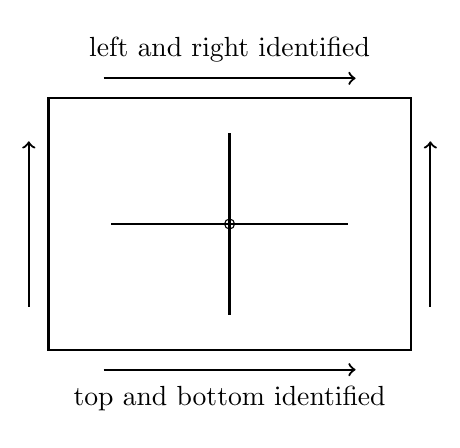
\begin{tikzpicture}[scale=1.0]
\draw[thick] (0,0) rectangle (4.6,3.2);

\draw[->,thick] (0.7,3.45)--(3.9,3.45);
\draw[->,thick] (0.7,-0.25)--(3.9,-0.25);

\draw[->,thick] (-0.25,0.55)--(-0.25,2.65);
\draw[->,thick] (4.85,0.55)--(4.85,2.65);

\draw[thick] (0.8,1.6)--(3.8,1.6);
\draw[thick] (2.3,0.45)--(2.3,2.75);

\draw (2.3,1.6) circle (1.8pt);

\draw (2.3,-0.62) node {top and bottom identified};
\draw (2.3,3.82) node {left and right identified};
\end{tikzpicture}\caption{직사각형의 마주 보는 변을 동일시해 만든 평탄한 토러스. 변은 경계가 아니다. 짝을 이루는 점들은 몫공간에서 같은 점이다.}\label{fig:c03-flat-torus}\end{figure}

\begin{classroomqa}\audiencequestion{그러면 우주는 평탄하면서도 유한할 수 있나요?}\lecturerresponse{그렇다. 평탄성은 계량에 관한 국소적 진술이고, 유한성은 위상에 관한 전역적 진술일 수 있다. 삼차원 토러스가 충분히 크면 전체 부피는 유한해도 우리가 관측할 수 있는 영역 전체에서 유클리드 공간처럼 보인다. \lecturetimestamp{01:13:37--01:17:59}}\end{classroomqa}

보편피복 공간의 그림을 보면 관측 가능한 결과가 분명해진다. 변들을 동일시하는 대신, 무한한 유클리드 평면에 기본 직사각형을 복사해 빈틈없이 깐다. 토러스 안의 단일 천체는 각 복사본에 한 번씩 나타난다. 삼차원에서는 복사본들이 주기적인 결정과 같은 배열을 이룬다.

\begin{classroomqa}\audiencequestion{우리도 모르는 사이에 토러스형 우주에 살 수 있나요?}\lecturerresponse{그렇다. 기본 셀이 빛이 우리에게 도달한 영역보다 크면 가능하다. 셀이 충분히 작다면 빛이 동일시된 경계를 통과할 수 있고, 우리는 서로 다른 방향에서 같은 은하의 반복된 상을 보거나 어쩌면 우리 주변 영역을 되풀이해 보게 될 수도 있다. 어느 경우든 국소 기하학은 평탄하게 유지된다. \lecturetimestamp{01:18:16--01:22:04}}\end{classroomqa}

\begin{classroomqa}\audiencequestion{구면은 대척점에서 멈추는데 토러스에서는 왜 반복되나요?}\lecturerresponse{구면에서는 주변 껍질이 \(r=\pi\)에서 실제로 수축해 사라진다. 모든 방사 방향이 대척점에서 만난다. 토러스에서는 선택한 직사각형 셀의 가장자리가 수축하지 않는다. 그 가장자리는 크기가 같은 반대편 가장자리와 동일시되므로, 이를 넘어가도 주기적인 좌표 기술 안에서 같은 공간이 계속 이어진다. \lecturetimestamp{01:22:06--01:23:02}}\end{classroomqa}

\section{공간에서 시공간으로}

이제 시간을 다시 도입하자. 광속이 \(c=1\)인 단위계에서 민코프스키 계량은 다음과 같다.
\begin{equation}
ds^2 = -dt^2 + dx^2 + dy^2 + dz^2.
\label{eq:c03-minkowski}
\end{equation}
부호 규약은 선택 사항이다. 중요한 것은 시간 항의 부호가 공간 항들과 반대라는 점이다. 빛은 영 궤적을 따른다.
\begin{equation}
ds^2 = 0.
\end{equation}
\(x\)방향으로만 움직인다면
\begin{equation}
-dt^2 + dx^2 = 0
\qquad\Rightarrow\qquad
dx = \pm dt.
\label{eq:c03-null-flat}
\end{equation}
두 부호는 빛이 단위 속력으로 왼쪽 또는 오른쪽으로 움직이는 경우를 나타낸다.

우주론에서는 고유시간 항 \(-dt^2\)을 그대로 두고 유클리드 공간 부분을 균질 공간 계량으로 바꾸며, 전체 척도가 시간에 따라 변하도록 한다. 이 척도인자를 \(a(t)\)으로 나타낸다. 이제 이것은 정적 비교에서 사용한 고정된 반지름 \(R_c\)이 아니라 동역학적 함수다.

그림으로 나타내기 쉬운 \(2+1\)차원 예로 다음을 생각하자.
\begin{equation}
ds^2 = -dt^2 + a(t)^2 d\Omega_2^2.
\label{eq:c03-two-plus-one}
\end{equation}
\(t\)가 고정될 때마다 공간은 반지름 \(a(t)\)인 \(2\)-구면이다. 이 구면들을 시간에 따라 쌓으면 시공간이 된다. 익숙한 \(3+1\)차원 구성은 다음과 같다.
\begin{equation}
ds^2 = -dt^2 + a(t)^2 d\Sigma^2,
\label{eq:c03-frw-general}
\end{equation}
여기서 \(d\Sigma^2\)는 시간에 따라 변하지 않는 단위 공간 계량이다. 단일 연결 공간의 세 경우는 다음과 같다.
\begin{align}
\text{flat:}\quad
ds^2&=-dt^2+a(t)^2\left(dx^2+dy^2+dz^2\right),\label{eq:c03-frw-flat}\\
\text{spherical:}\quad
ds^2&=-dt^2+a(t)^2d\Omega_3^2,\label{eq:c03-frw-spherical}\\
\text{hyperbolic:}\quad
ds^2&=-dt^2+a(t)^2dh_3^2.\label{eq:c03-frw-hyperbolic}
\end{align}
공변 좌표 사이의 상대적 척도는 \(a(t)\)가 변하는 동안 고정되어 있다. 구면 및 쌍곡 정규화에서는 \(a(t)\)가 순간적인 곡률반지름이기도 하다. 평탄한 경우에는 공변 좌표를 재정의해 절대 정규화를 흡수할 수 있다.

중력장 방정식을 적용하기 전에도 허블 법칙을 얻을 수 있다. 좌표 간격 \(\chi\)가 고정된 가까운 두 공변점에 주목하자. 이들의 물리적 거리는
\begin{equation}
D(t)=a(t)\chi.
\label{eq:c03-comoving-distance}
\end{equation}
\(\chi\)을 고정한 채 미분하면
\begin{equation}
V=\dot D=\dot a(t)\chi.
\end{equation}
\(\chi\)을 소거하면
\begin{equation}
V = \frac{\dot a}{a} D.
\label{eq:c03-hubble-law}
\end{equation}
따라서
\begin{equation}
H = \frac{\dot a}{a}.
\label{eq:c03-hubble-parameter}
\end{equation}
이는 균질한 팽창이나 수축에 대한 운동학적 항등식이다. 세 공간 기하학 모두에서 성립하며, \(\dot a>0\)이면 멀어지고 \(\dot a<0\)이면 가까워진다.

기하학만으로는 \(a(t)\)를 결정할 수 없다. 다음과 같은 함수는
\begin{equation}
a(t)\propto t^{2/3},
\qquad
a(t)\propto t^{1/2},
\qquad
a(t)\propto e^{Ht}
\end{equation}
모두 균질 계량의 가정에 들어맞지만, 서로 다른 우주 물질과 에너지의 구성을 나타낸다. 일반 상대성 이론은 이들 가운데 하나를 선택하는 동역학 방정식을 제공한다. 그 결과 얻는 프리드만 방정식은 평탄한 경우, 구면인 경우, 쌍곡선인 경우를 앞서 전개한 뉴턴 우주론의 에너지가 0인 경우, 음의 경우, 양의 경우와도 연결해 준다.

\begin{classroomqa}
\audiencequestion{기하학과 우주의 진화가 이 모형들보다 훨씬 더 복잡할 수도 있나요?}
\lecturerresponse{물론입니다. 균질성과 등방성은 제약이 큰 가정입니다. 이 가정들은 자연스럽고, 큰 규모에서 관측 결과와 잘 맞으며, 수학적으로 다루기 쉬워 채택되었습니다. 훨씬 더 복잡한 기하학과 진화도 존재합니다. 중요한 동역학적 질문은 처음에 불규칙했던 모형의 광범위한 부류가 이처럼 단순한 균질 형태 가운데 하나로 진화하는가 하는 것입니다. \lecturetimestamp{01:36:00--01:36:50}}
\end{classroomqa}

\begin{classroomqa}
\audiencequestion{\(3\)-구면은 4차원 물체의 경계인가요?}
\lecturerresponse{매장으로 표현할 수는 있지만, 우주론적 공간은 \(3\)-구면 자체입니다. 본질적으로 세 차원이며 경계는 없습니다. 4차원 유클리드 그림은 선택적인 보조 수단일 뿐이고, 방정식~\eqref{eq:c03-three-sphere}만으로 이미 기하가 완전히 정의됩니다. \lecturetimestamp{01:36:55--01:37:59}}
\end{classroomqa}

\begin{classroomqa}
\audiencequestion{곡률을 검사하는 데 필요한 거리를 구하는 방법은 광도뿐인가요?}
\lecturerresponse{아닙니다. 스펙트럼선으로 적색편이를 알아내고, 가까운 거리 사다리로 허블 관계를 보정하며, 초신성으로 대략 표준적인 광도를 얻습니다. 이 방법들은 각각 따로 신뢰하는 것이 아니라 서로 대조해 검증합니다. 역제곱 광도 법칙조차 기하학에 좌우됩니다. 빛의 파면의 면적이 \(r^2\), \(\sin^2r\) 또는 \(\sinh^2r\)로 정해지기 때문입니다. 여러 관측량이 서로 일치한다는 점이 우주가 거의 평탄하다는 결론을 뒷받침합니다. \lecturetimestamp{01:38:00--01:41:07}}
\end{classroomqa}

\section{기억해 둘 점}

균질 우주의 기하학은 임의의 관측자를 중심으로 한 껍질의 크기가 어떻게 증가하는지 살펴보면 알 수 있다.
\begin{equation}
f(r)=
\begin{cases}
r, & \text{flat space},\\
\sin r, & \text{positive curvature},\\
\sinh r, & \text{negative curvature}.
\end{cases}
\end{equation}
공간 계량은 \(dr^2+f(r)^2d\Omega_{n-1}^2\)이다. 같은 함수가 각 크기와 껍질 안에 존재하는 천체의 수도 결정하므로, 곡률은 관측 가능한 의미를 직접 갖는다. 곡률 반지름이 크면 이러한 차이가 국소적으로 드러나지 않으며, 토러스형 동일시를 보면 국소 곡률만으로는 전체 크기나 위상을 결정할 수 없다는 점을 알 수 있다.

\(-dt^2\)와 공통 인자 \(a(t)^2\)를 더하면 균질한 세 공간 계량 가운데 어느 것이든 우주 시공간이 된다. 그러면 곧바로 \(V=HD\)와 \(H=\dot a/a\)을 얻지만, \(a(t)\)는 정해지지 않는다. 따라서 다음 단계는 기하학을 더 다루는 일이 아니다. 동역학 문제를 풀어야 한다. 아인슈타인 방정식을 이용해 물질, 복사, 곡률 및 다른 형태의 에너지가 척도 인자를 어떻게 진화시키는지 결정해야 한다.
